\section{Diagramy Przypadków Użycia}

\subsection{Opis aktorów}
\textit{Należy wypełnić opis wszystkich aktorów, wchodzących w interakcje z systemem. Jeśli to uzasadnione należy dodać diagram prezentujący związki pomiędzy aktorami, np. dziedziczenie}

\begin{enumerate}
	\item \textbf{Użytkownik bez stałego konta.} Typ użytkownika, którego konto jest tworzone podczas połączenia z serwerem czatu oraz 
		niszczone po jego zakończeniu. Podczas łączenia z czatem, nie będzie musiał się autoryzować przy użyciu hasła, a deklarować
		tylko unikalną nazwę, nie powtarzającą się z nazwą innego użytkownika, posiadającego konto na danym serwerze czatu. Ten typ
		konta jest przeznaczony dla osób, zainteresowanych dołączeniem do dyskusji na czacie bez dodatkowych zobowiązań. Jest aktorem aktywnym
		i głównym.
		
	\item \textbf{Użytkownik stały.} Typ użytkownika, którego konto jest utrzymywane przez serwer pomiędzy połączeniami do czatu. W
		zamierzeniu, adresatami takiego rozwiązania mają być stali bywalcy serwera, którzy chcą mieć zarezerwowaną określoną nazwę
		dla siebie i uniknąć ewentualnego podszywania się. Stąd każdorazowo, przed rozpoczęciem sesji połączenia z serwerem, muszą się
		dodatkowo autoryzować przy użyciu hasła. Równocześnie, ich nazwa jest zarezerwowana wyłącznie do jego użytku oraz niedostępna
		dla użytkowników tymczasowych.  Jest aktorem aktywnym i głównym.
		
	\item \textbf{Administrator.} To użytkownik stały, który jest dodatkowo wyróżniony i posiada uprawienia do szeroko pojętego 
		zarządzania serwerem (w tym - pozostałymi użytkownikami). Nie wyróżnia się wśród administratorów żadnych dodatkowych, szczególnych
		ról (np. superadministrator, właściciel).  Jest aktorem aktywnym i głównym.
		
	\item \textbf{Użytkownik czatu.} W tej kategorii mieszczą się wszyscy
	użytkownicy serwera, niezależnie od tego, czy mają stałe czy też nie.

\end{enumerate}

\newpage
\subsection{Diagram Przypadków Użycia}

Diagram przypadków użycia jest pokazany na rysunku 1 \ref{diagram_przypadkow_uzycia} \nameref{diagram_przypadkow_uzycia} na stronie \pageref{diagram_przypadkow_uzycia}.
\begin{figure}[!htp]
	\centering
	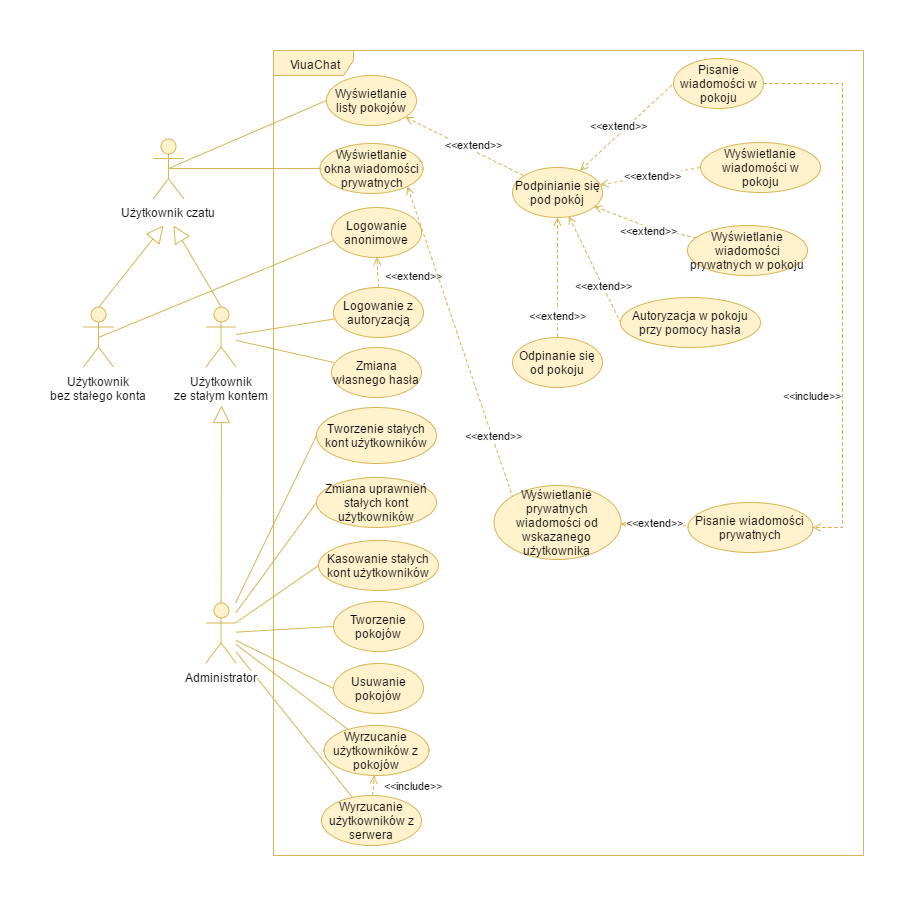
\includegraphics[width=\textwidth]{chat/fig/viuavm-dpu-v2}
	\caption{Diagram przypadków użycia}
	\label{diagram_przypadkow_uzycia}
\end{figure}

\newpage

\subsection{Opis przypadków użycia}

Poniżej opisano przypadki użycia ujęte na powyższym diagramie.

{\footnotesize

\vspace{2em}

\begin{tabular}{ | l | l | }
	\hline
		\textbf{Identyfikator} & 
		UC-01
		\\
		
	\hline
		\textbf{Nazwa} & 
		Logowanie anonimowe
		\\
		
	\hline
		\textbf{Aktorzy} & \parbox[t]{11cm}{
			Użytkownik bez stałego konta
		}\\
		 
	\hline
		\parbox[t]{4cm}{\textbf{Streszczenie}} & \parbox[t]{11cm}{
			Użytkownik rozpoczyna korzystanie z czatu pod wybraną nazwą
			użytkownika, ale bez konieczności podawania hasła.
			
		}\\
		
	\hline
		\parbox[t]{4cm}{\textbf{Warunek wstępny}} & \parbox[t]{11cm}{
			Użytkownik nie ma rozpoczętej sesji połączenia z serwerem
		}
		\\
		
	\hline
		\parbox[t]{4cm}{\textbf{Wyjątki}} & \parbox[t]{11cm}{
			\begin{itemize}
				\item Użytkownik ma już wcześniej rozpoczętą
				 sesję z serwerem
			\end{itemize}
			
		}
		\\

	\hline
		\parbox[t]{4cm}{\textbf{Scenariusz podstawowy}} & \parbox[t]{11cm}{
			\begin{enumreq}
				\item Użytkownik wprowadza nazwę użytkownika i zatwierdza
				\item System sprawdza czy nazwa użytkownika jest wolna
				\item Gdy nazwa jest wolna, serwer rozpoczyna sesję
				z użytkownikiem
			\end{enumreq}
		}
		\\
		
	\hline
		\parbox[t]{4cm}{\textbf{Scenariusze alternatywne}} & \parbox[t]
		{11cm}{
			\begin{enumreq}
				\item Gdy nazwa użytkownika jest zajęta (przez zalogowanego
				użytkownika lub stałe konto użytkownika), logowanie nie
				powiedzie się.
			\end{enumreq}
		}
		\\
		
	\hline
		\parbox[t]{4cm}{\textbf{Warunek końcowy}} & \parbox[t]{11cm}{
			Użytkownik ma rozpoczętą sesję z serwerem.
		}
		\\
		
	\hline
		\parbox[t]{4cm}{\textbf{Komentarz}} & \parbox[t]{11cm}{
			\textit{Nie zamieszczono}
		}
		\\

	\hline
\end{tabular}

\vspace{2em}

\begin{tabular}{ | l | l | }
	\hline
		\textbf{Identyfikator} & 
		UC-02
		\\
		
	\hline
		\textbf{Nazwa} & 
		Logowanie z autoryzacją
		\\
		
	\hline
		\textbf{Aktorzy} & \parbox[t]{11cm}{
			Użytkownik ze stałym kontem
		}\\
		 
	\hline
		\parbox[t]{4cm}{\textbf{Streszczenie}} & \parbox[t]{11cm}{
			Użytkownik rozpoczyna korzystanie z czatu z wykorzystaniem
			stałego konta, uwierzytelniając hasłem, czy ma prawo do
			jego wykorzystywania.
			
		}\\
		
	\hline
		\parbox[t]{4cm}{\textbf{Warunek wstępny}} & \parbox[t]{11cm}{
			\begin{enumerate}
				\item Użytkownik nie ma rozpoczętej sesji połączenia 
				z serwerem.
				\item Użytkownik posiada założone stałe konto na serwerze
			\end{enumerate}
			
		}
		\\
		
	\hline
		\parbox[t]{4cm}{\textbf{Wyjątki}} & \parbox[t]{11cm}{
			\begin{itemize}
				\item Użytkownik ma już wcześniej rozpoczętą
				 sesję z serwerem
			\end{itemize}
			
		}
		\\

	\hline
		\parbox[t]{4cm}{\textbf{Scenariusz podstawowy}} & \parbox[t]{11cm}{
			\begin{enumerate}
				\item Użytkownik wprowadza nazwę użytkownika, hasło 
				i zatwierdza
				\item Gdy istnieje stałe konto o wskazanej nazwie, a
				podane hasło jest z nim zgodne, wówczas serwer rozpoczyna
				sesję z użytkownikiem.
			\end{enumerate}
		}
		\\
		
	\hline
		\parbox[t]{4cm}{\textbf{Scenariusze alternatywne}} & \parbox[t]
		{11cm}{
			\begin{enumerate}
				\item Gdy nie istnieje stałe konto użytkownika o podanej
				nazwie, logowanie nie powiedzie się
				\item Gdy podane hasło nie jest zgodne z hasłem do
				konta użytkownika o podanej nazwie, logowanie nie powiedzie
				się.
			\end{enumerate}
		}
		\\
		
	\hline
		\parbox[t]{4cm}{\textbf{Warunek końcowy}} & \parbox[t]{11cm}{
			Użytkownik ma rozpoczętą sesję z serwerem.
		}
		\\
		
	\hline
		\parbox[t]{4cm}{\textbf{Komentarz}} & \parbox[t]{11cm}{
			\textit{Nie zamieszczono}
		}
		\\

	\hline
\end{tabular}

\vspace{2em}

\begin{tabular}{ | l | l | }
	\hline
		\textbf{Identyfikator} & 
		UC-03
		\\
		
	\hline
		\textbf{Nazwa} & 
		Zmiana własnego hasła
		\\
		
	\hline
		\textbf{Aktorzy} & \parbox[t]{11cm}{
			Użytkownik ze stałym kontem
		}\\
		 
	\hline
		\parbox[t]{4cm}{\textbf{Streszczenie}} & \parbox[t]{11cm}{
			Użytkownik zmienia hasło, używane podczas logowania z użyciem
			stałego konta.
			
		}\\
		
	\hline
		\parbox[t]{4cm}{\textbf{Warunek wstępny}} & \parbox[t]{11cm}{
			\begin{enumreq}
				\item Użytkownik ma rozpoczętą sesję z serwerem
				\item Użytkownik jest użytkownikiem ze stałym kontem
			\end{enumreq}
		}
		\\
		
	\hline
		\parbox[t]{4cm}{\textbf{Wyjątki}} & \parbox[t]{11cm}{
			\textit{Brak}
			
		}
		\\

	\hline
		\parbox[t]{4cm}{\textbf{Scenariusz podstawowy}} & \parbox[t]{11cm}{
			\begin{enumreq}
				\item Użytkownik wprowadza dotychczasowe hasło i dwukrotnie
				wprowadza nowe hasło.
				\item System sprawdza, czy dotychczasowe hasło zgadza się
				z tym, które jest przypisane do konta, z którego korzysta
				obecnie użytkownik
				\item System sprawdza czy nowe hasło jest za każdym razem
				takie same
				\item Hasło zostaje zmienione
				\item Użytkownik uzyskuje informację o sukcesie zmiany
			\end{enumreq}
		}
		\\
		
	\hline
		\parbox[t]{4cm}{\textbf{Scenariusze alternatywne}} & \parbox[t]
		{11cm}{
			\begin{enumreq}
				\item Gdy hasło obecne nie jest prawidłowe, zmiana nie
				powiedzie się.
				\item Gdy nowe hasła się różnią, zmiana nie powiedzie się.
				\item Gdy nowe hasło jest zbyt krótkie lub puste, zmiana
				nie powiedzie się.
				\item W razie niepowodzenia, pola haseł (obecnego i dwóch
				nowych) zostają wyczyszczone.
			\end{enumreq}
		}
		\\
		
	\hline
		\parbox[t]{4cm}{\textbf{Warunek końcowy}} & \parbox[t]{11cm}{
			Użytkownik ma zmienione hasło.
		}
		\\
		
	\hline
		\parbox[t]{4cm}{\textbf{Komentarz}} & \parbox[t]{11cm}{
			\textit{Nie zamieszczono}
		}
		\\

	\hline
\end{tabular}

\vspace{2em}

\begin{tabular}{ | l | l | }
	\hline
		\textbf{Identyfikator} & 
		UC-04
		\\
		
	\hline
		\textbf{Nazwa} & 
		Wyświetlanie listy pokojów
		\\
		
	\hline
		\textbf{Aktorzy} & \parbox[t]{11cm}{
			Użytkownik czatu
		}\\
		 
	\hline
		\parbox[t]{4cm}{\textbf{Streszczenie}} & \parbox[t]{11cm}{
			Użytkownik uzyskuje wgląd do listy pokojów z której może
			wybrać ten, do którego chce się podpiąć.
			
		}\\
		
	\hline
		\parbox[t]{4cm}{\textbf{Warunek wstępny}} & \parbox[t]{11cm}{
			\begin{enumreq}
				\item Użytkownik ma rozpoczętą sesję z serwerem
			\end{enumreq}
				
		}
		\\
		
	\hline
		\parbox[t]{4cm}{\textbf{Wyjątki}} & \parbox[t]{11cm}{
			\begin{enumreq}
				\item Użytkownik nie może być podpięty do żadnego pokoju
			\end{enumreq}
			\textit{Brak}
			
		}
		\\

	\hline
		\parbox[t]{4cm}{\textbf{Scenariusz podstawowy}} & \parbox[t]{11cm}{
			\begin{enumreq}
				\item Użytkownik wybiera z górnego menu opcję ,,Pokoje''
				\item Użytkownik wybiera jeden z pokojów, do którego chce
				się wpiąć.
			\end{enumreq}
		}
		\\
		
	\hline
		\parbox[t]{4cm}{\textbf{Scenariusze alternatywne}} & \parbox[t]
		{11cm}{
			\begin{enumreq}
				\item Wiadomości prywatne są wysyłane z okna czatu w 
				specyficzny sposób (patrz UC-10)
			\end{enumreq}
		}
		\\
		
	\hline
		\parbox[t]{4cm}{\textbf{Warunek końcowy}} & \parbox[t]{11cm}{
			Użytkownik wybrał pokój do wpięcia się.
		}
		\\
		
	\hline
		\parbox[t]{4cm}{\textbf{Komentarz}} & \parbox[t]{11cm}{
			\textit{Nie zamieszczono}
		}
		\\

	\hline
\end{tabular}

\vspace{2em}

\begin{tabular}{ | l | l | }
	\hline
		\textbf{Identyfikator} & 
		UC-05
		\\
		
	\hline
		\textbf{Nazwa} & 
		Podpinanie się pod pokój
		\\
		
	\hline
		\textbf{Aktorzy} & \parbox[t]{11cm}{
			Użytkownik czatu
		}\\
		 
	\hline
		\parbox[t]{4cm}{\textbf{Streszczenie}} & \parbox[t]{11cm}{
			Użytkownik czatu, po wybraniu pokoju z listy pokojów, jest
			do niego wpinany.
			
		}\\
		
	\hline
		\parbox[t]{4cm}{\textbf{Warunek wstępny}} & \parbox[t]{11cm}{
			\begin{enumreq}
				\item Użytkownik wybrał pokój z listy pokojów
			\end{enumreq}
				
		}
		\\
		
	\hline
		\parbox[t]{4cm}{\textbf{Wyjątki}} & \parbox[t]{11cm}{
			\begin{enumreq}
				\item Użytkownik nie może być już wcześniej wpięty
				do żadnego pokoju.
			\end{enumreq}
			
		}
		\\

	\hline
		\parbox[t]{4cm}{\textbf{Scenariusz podstawowy}} & \parbox[t]{11cm}{
			\begin{enumreq}
				\item Użytkownik wybiera pokój z listy
				\item Serwer weryfikuje, czy użytkownik nie był już
				wcześniej wpięty do innego pokoju
				\item Jeżeli użytkownik pozostawał wcześniej niepodpięty,
				serwer weryfikuje, czy pokój jest zabezpieczony hasłem
				\item Jeżeli pokój jest niezabezpieczony, następuje
				podpięcie użytkownika pod wybrany pokój.
			\end{enumreq}
		}
		\\
		
	\hline
		\parbox[t]{4cm}{\textbf{Scenariusze alternatywne}} & \parbox[t]
		{11cm}{
			\begin{enumreq}
				\item Gdy wybrany został pokój zabezpieczony hasłem,
				to następuje przełączenie na scenariusz UC-11
				\item Gdy użytkownik był wcześniej wpięty do innego pokoju,
				ponowne podpięcie kończy się niepowodzeniem.
			\end{enumreq}
		}
		\\
		
	\hline
		\parbox[t]{4cm}{\textbf{Warunek końcowy}} & \parbox[t]{11cm}{
			Użytkownik został podpięty pod pokój.
		}
		\\
		
	\hline
		\parbox[t]{4cm}{\textbf{Komentarz}} & \parbox[t]{11cm}{
			\textit{Nie zamieszczono}
		}
		\\

	\hline
\end{tabular}

\vspace{2em}

\begin{tabular}{ | l | l | }
	\hline
		\textbf{Identyfikator} & 
		UC-06
		\\
		
	\hline
		\textbf{Nazwa} & 
		Odpinanie się od pokoju
		\\
		
	\hline
		\textbf{Aktorzy} & \parbox[t]{11cm}{
			Użytkownik czatu
		}\\
		 
	\hline
		\parbox[t]{4cm}{\textbf{Streszczenie}} & \parbox[t]{11cm}{
			Użytkownik, który był wcześniej wpięty do pokoju, może się
			od niego odpiąć, aby wpiąć się do innego pokoju lub po prostu
			zrezygnować z dalszej konwersacji.
			
		}\\
		
	\hline
		\parbox[t]{4cm}{\textbf{Warunek wstępny}} & \parbox[t]{11cm}{
			\begin{enumreq}
				\item Użytkownik ma rozpoczętą sesję z serwerem
				\item Użytkownik jest podpięty do pokoju
			\end{enumreq}
				
		}
		\\
		
	\hline
		\parbox[t]{4cm}{\textbf{Wyjątki}} & \parbox[t]{11cm}{
			\textit{Brak}
			
		}
		\\

	\hline
		\parbox[t]{4cm}{\textbf{Scenariusz podstawowy}} & \parbox[t]{11cm}{
			\begin{enumreq}
				\item Użytkownik wybiera przycisk ,,Opuść pokój''.
				\item Serwer weryfikuje, czy użytkownik nadal jest podpięty
				pod pokój
				\item Jeżeli użytkownik jest nadal podpięty, następuje
				odpięcie
				\item Użytkownikowi zostaje przekierowany do listy pokojów
			\end{enumreq}
		}
		\\
		
	\hline
		\parbox[t]{4cm}{\textbf{Scenariusze alternatywne}} & \parbox[t]
		{11cm}{
			\begin{enumreq}
				\item Gdy użytkownik pozostawał wcześniej niepodpięty, akcja
				kończy się niepowodzeniem.
			\end{enumreq}
		}
		\\
		
	\hline
		\parbox[t]{4cm}{\textbf{Warunek końcowy}} & \parbox[t]{11cm}{
			Użytkownik zostaje odpięty od pokoju.
		}
		\\
		
	\hline
		\parbox[t]{4cm}{\textbf{Komentarz}} & \parbox[t]{11cm}{
			\textit{Nie zamieszczono}
		}
		\\

	\hline
\end{tabular}

\vspace{2em}

\begin{tabular}{ | l | l | }
	\hline
		\textbf{Identyfikator} & 
		UC-07
		\\
		
	\hline
		\textbf{Nazwa} & 
		Pisanie wiadomości w pokoju
		\\
		
	\hline
		\textbf{Aktorzy} & \parbox[t]{11cm}{
			Użytkownik czatu
		}\\
		 
	\hline
		\parbox[t]{4cm}{\textbf{Streszczenie}} & \parbox[t]{11cm}{
			Użytkownik może napisać wiadomość w pokoju czatu, którą zobaczą
			inni użytkownicy podpięci do tego pokoju (włącznie z jej nadawcą)	
		}\\
		
	\hline
		\parbox[t]{4cm}{\textbf{Warunek wstępny}} & \parbox[t]{11cm}{
			\begin{enumreq}
				\item Użytkownik ma rozpoczętą sesję z serwerem
				\item Użytkownik jest podpięty do pokoju
			\end{enumreq}
				
		}
		\\
		
	\hline
		\parbox[t]{4cm}{\textbf{Wyjątki}} & \parbox[t]{11cm}{
			\textit{Brak}
			
		}
		\\

	\hline
		\parbox[t]{4cm}{\textbf{Scenariusz podstawowy}} & \parbox[t]{11cm}{
			\begin{enumreq}
				\item Użytkownik pisze wiadomość w polu tekstowym
				pod wiadomościami czatu
				\item Po zatwierdzeniu wiadomości do wysyłki, pole tekstowe
				jest czyszczone
				\item Gdy użytkownik jest nadal podpięty do pokoju, wiadomość
				zostaje wpisana do listy wiadomości i rozesłana do wszystkich
				użytkowników
			\end{enumreq}
		}
		\\
		
	\hline
		\parbox[t]{4cm}{\textbf{Scenariusze alternatywne}} & \parbox[t]
		{11cm}{
			\begin{enumreq}
				\item Gdy użytkownik nie był wpięty do pokoju w momencie
				wysyłania wiadomości, wysyłka kończy się niepowodzeniem
				\item Gdy wiadomość jest poprzedzona znakiem ..\#'', to
				jest realizowany scenariusz UC-11
			\end{enumreq}
		}
		\\
		
	\hline
		\parbox[t]{4cm}{\textbf{Warunek końcowy}} & \parbox[t]{11cm}{
			Wiadomość została zaakceptowania do rozesłania przez serwer
		}
		\\
		
	\hline
		\parbox[t]{4cm}{\textbf{Komentarz}} & \parbox[t]{11cm}{
			\textit{Nie zamieszczono}
		}
		\\

	\hline
\end{tabular}

\vspace{2em}

\begin{tabular}{ | l | l | }
	\hline
		\textbf{Identyfikator} & 
		UC-09
		\\
		
	\hline
		\textbf{Nazwa} & 
		Wyświetlanie wiadomości w pokoju
		\\
		
	\hline
		\textbf{Aktorzy} & \parbox[t]{11cm}{
			Użytkownik czatu
		}\\
		 
	\hline
		\parbox[t]{4cm}{\textbf{Streszczenie}} & \parbox[t]{11cm}{
			Użytkownicy w pokoju otrzymują wiadomości, które są do niego
			wysyłane.
			
		}\\
		
	\hline
		\parbox[t]{4cm}{\textbf{Warunek wstępny}} & \parbox[t]{11cm}{
			\begin{enumreq}
				\item Serwer przyjął wiadomość do rozesłania w ramach pokoju
				\item Użytkownik czatu został wpięty do pokoju
			\end{enumreq}
				
		}
		\\
		
	\hline
		\parbox[t]{4cm}{\textbf{Wyjątki}} & \parbox[t]{11cm}{
			\begin{enumreq}
				\item Wiadomości prywatne w oknie pokoju są wyświetlane
				inaczej (patrz UC-13)
			\end{enumreq}
			
		}
		\\

	\hline
		\parbox[t]{4cm}{\textbf{Scenariusz podstawowy}} & \parbox[t]{11cm}{
			\begin{enumreq}
				\item Serwer rozysła nową wiadomość do wszystkich
				użytkowników podpiętych do pokoju czatu
				\item Użytkownikowi zostaje pokazana nowa wiadomość
				u dołu okna pokoju
			\end{enumreq}
		}
		\\
		
	\hline
		\parbox[t]{4cm}{\textbf{Scenariusze alternatywne}} & \parbox[t]
		{11cm}{
			\begin{enumreq}
				\item Uzytkownikowi, który zostaje nowo podpięty do pokoju,
				pokazywane jest 10 wiadomości wysłanych tuż przed dołączeniem
				do tego pokoju.
			\end{enumreq}
		}
		\\
		
	\hline
		\parbox[t]{4cm}{\textbf{Warunek końcowy}} & \parbox[t]{11cm}{
			Użytkownik widzi wiadomość w oknie pokoju.
		}
		\\
		
	\hline
		\parbox[t]{4cm}{\textbf{Komentarz}} & \parbox[t]{11cm}{
			\textit{Nie zamieszczono}
		}
		\\

	\hline
\end{tabular}

\vspace{2em}

\begin{tabular}{ | l | l | }
	\hline
		\textbf{Identyfikator} & 
		UC-10
		\\
		
	\hline
		\textbf{Nazwa} & 
		Wyświetlanie prywatnych wiadomości w pokoju
		\\
		
	\hline
		\textbf{Aktorzy} & \parbox[t]{11cm}{
			Użytkownik czatu
		}\\
		 
	\hline
		\parbox[t]{4cm}{\textbf{Streszczenie}} & \parbox[t]{11cm}{
			Użytkownik widzi wiadomości prywatne, skierowane do niego przez
			innego użytkownika podpiętego do tego samego pokoju. Wiadomości
			tych nie widzi żaden inny użytkownik podpięty do pokoju, oprócz
			jej nadawcy i odbiorcy.
			
		}\\
		
	\hline
		\parbox[t]{4cm}{\textbf{Warunek wstępny}} & \parbox[t]{11cm}{
			\begin{enumreq}
				\item Użytkownik ma rozpoczętą sesję z serwerem
				\item Użytkownik jest podpięty do pokoju
				\item Użytkownik wysłał wiadomość do pokoju (patrz UC-07)
				poprzedzoną znakiem ,,\#''
			\end{enumreq}
				
		}
		\\
		
	\hline
		\parbox[t]{4cm}{\textbf{Wyjątki}} & \parbox[t]{11cm}{
			\textit{Brak}
			
		}
		\\

	\hline
		\parbox[t]{4cm}{\textbf{Scenariusz podstawowy}} & \parbox[t]{11cm}{
			\begin{enumreq}
				\item Użytkownik wysyła do pokoju wiadomość poprzedzoną
				znakiem ,,\#''
				\item Serwer sprawdza, czy przed treścią wiadomości znajduje
				się łańcuch znaków będący prawidłową nazwą użytkownika
				\item Jeżeli forma nazwy jest prawidłowa, serwer sprawdza,
				czy użytkownik wskazany na początku wiadomości jest podpięty
				do pokoju
				\item Jeżeli użytkownik jest podpięty do pokoju, wiadomość
				zostaje przyjęta przez serwer jako wiadomość prywatna
			\end{enumreq}
		}
		\\
		
	\hline
		\parbox[t]{4cm}{\textbf{Scenariusze alternatywne}} & \parbox[t]
		{11cm}{
			\begin{enumreq}
				\item Gdy nazwa użytkownika odbiorcy ma nieprawidłową formę
				bądź odbiorca nie jest podpięty pod pokój, wiadomość nie
				zostanie przyjęta przez serwer i wysyłka zakończy się
				niepowodzeniem
			\end{enumreq}
		}
		\\
		
	\hline
		\parbox[t]{4cm}{\textbf{Warunek końcowy}} & \parbox[t]{11cm}{
			Wiadomość prywatna została przyjęta przez serwer.
		}
		\\
		
	\hline
		\parbox[t]{4cm}{\textbf{Komentarz}} & \parbox[t]{11cm}{
			\textit{Nie zamieszczono}
		}
		\\

	\hline
\end{tabular}

\vspace{2em}

\begin{tabular}{ | l | l | }
	\hline
		\textbf{Identyfikator} & 
		UC-11
		\\
		
	\hline
		\textbf{Nazwa} & 
		Autoryzacja w pokoju przy pomocy hasła
		\\
		
	\hline
		\textbf{Aktorzy} & \parbox[t]{11cm}{
			Użytkownik czatu
		}\\
		 
	\hline
		\parbox[t]{4cm}{\textbf{Streszczenie}} & \parbox[t]{11cm}{
			Użytkownik, przed podpięciem do pokoju zabezpieczonego hasłem,
			musi podać jego hasło.
			
		}\\
		
	\hline
		\parbox[t]{4cm}{\textbf{Warunek wstępny}} & \parbox[t]{11cm}{
			\begin{enumreq}
				\item Użytkownik ma rozpoczętą sesję z serwerem
				\item Użytkownik wybrał pokój do podpięcia i może się do
				niego podpiąć (patrz UC-05), pokój jest zabezpieczony 
				hasłem
			\end{enumreq}
				
		}
		\\
		
	\hline
		\parbox[t]{4cm}{\textbf{Wyjątki}} & \parbox[t]{11cm}{
			\textit{Brak}
			
		}
		\\

	\hline
		\parbox[t]{4cm}{\textbf{Scenariusz podstawowy}} & \parbox[t]{11cm}{
			\begin{enumreq}
				\item Użytkownik wpisuje hasło do pokoju
				\item Gdy podane hasło jest prawidłowe, użytkownik
				zostaje podpięty
			\end{enumreq}
		}
		\\
		
	\hline
		\parbox[t]{4cm}{\textbf{Scenariusze alternatywne}} & \parbox[t]
		{11cm}{
			\begin{enumreq}
				\item Gdy podane hasło nie jest prawidłowe, użytkownik
				zoostaje ponownie poproszony o jego podanie
				\item Gdy użytkownik zrezygnuje z podania hasła, pozostanie
				niepodpięty
				\item Gdy pokój nie jest już zabezpieczony hasłem, podpięcie
				następuje niezależnie od wpisanego hasła.
			\end{enumreq}
		}
		\\
		
	\hline
		\parbox[t]{4cm}{\textbf{Warunek końcowy}} & \parbox[t]{11cm}{
			Użytkownik został wpięty do pokoju
		}
		\\
		
	\hline
		\parbox[t]{4cm}{\textbf{Komentarz}} & \parbox[t]{11cm}{
			\textit{Nie zamieszczono}
		}
		\\

	\hline
\end{tabular}

\vspace{2em}

\begin{tabular}{ | l | l | }
	\hline
		\textbf{Identyfikator} & 
		UC-12
		\\
		
	\hline
		\textbf{Nazwa} & 
		Wyświetlanie okna wiadomości prywatnych
		\\
		
	\hline
		\textbf{Aktorzy} & \parbox[t]{11cm}{
			Użytkownik czatu
		}\\
		 
	\hline
		\parbox[t]{4cm}{\textbf{Streszczenie}} & \parbox[t]{11cm}{
			Użytkownik może zobaczyć okno z wiadomościami prywatnymi
			(niezależnie od tego czy zostały wysłane z pokoju czy z okna
			wiadomości prywatnych), pogrupowane wg ich nadawców/odbiorców
			
		}\\
		
	\hline
		\parbox[t]{4cm}{\textbf{Warunek wstępny}} & \parbox[t]{11cm}{
			\begin{enumreq}
				\item Użytkownik ma rozpoczętą sesję z serwerem
			\end{enumreq}
				
		}
		\\
		
	\hline
		\parbox[t]{4cm}{\textbf{Wyjątki}} & \parbox[t]{11cm}{
			\textit{Brak}
			
		}
		\\

	\hline
		\parbox[t]{4cm}{\textbf{Scenariusz podstawowy}} & \parbox[t]{11cm}{
			\begin{enumreq}
				\item Użytkownik wybiera z menu opcję ,,PW''
				\item Użytkownikowi zostaje pokazana lista nazw użytkowników
				od których otrzymał lub którym wysyłał wiadomości prywatne
			\end{enumreq}
		}
		\\
		
	\hline
		\parbox[t]{4cm}{\textbf{Scenariusze alternatywne}} & \parbox[t]
		{11cm}{
			\begin{enumreq}
				\item Gdy użytkownik nie wysłał ani nie odebrał żadnych
				wiadomości prywatnych, lista nazw użytkowników będzie pusta.
			\end{enumreq}
		}
		\\
		
	\hline
		\parbox[t]{4cm}{\textbf{Warunek końcowy}} & \parbox[t]{11cm}{
			Użytkownik zobaczy listę nazw użytkowników, od których
			otrzymał lub którym wysłał wiadomości prywatne
		}
		\\
		
	\hline
		\parbox[t]{4cm}{\textbf{Komentarz}} & \parbox[t]{11cm}{
			\textit{Nie zamieszczono}
		}
		\\

	\hline
\end{tabular}

\vspace{2em}

\begin{tabular}{ | l | l | }
	\hline
		\textbf{Identyfikator} & 
		UC-13
		\\
		
	\hline
		\textbf{Nazwa} & 
		Wyświetlanie prywatnych wiadomości od wskazanego użytkownika
		\\
		
	\hline
		\textbf{Aktorzy} & \parbox[t]{11cm}{
			Użytkownik czatu
		}\\
		 
	\hline
		\parbox[t]{4cm}{\textbf{Streszczenie}} & \parbox[t]{11cm}{
			Użytkownik musi wybrać konkretnego innego użytkownika,
			aby zobaczyć jego wiadomości (tj. tych, których jest
			nadawcą/odbiorcą)
			
		}\\
		
	\hline
		\parbox[t]{4cm}{\textbf{Warunek wstępny}} & \parbox[t]{11cm}{
			\begin{enumreq}
				\item Użytkownik wybrał nazwę użytkownika w oknie wiadomości
				 prywatnych
			\end{enumreq}
				
		}
		\\
		
	\hline
		\parbox[t]{4cm}{\textbf{Wyjątki}} & \parbox[t]{11cm}{
			\textit{Brak}
			
		}
		\\

	\hline
		\parbox[t]{4cm}{\textbf{Scenariusz podstawowy}} & \parbox[t]{11cm}{
			\begin{enumreq}
				\item Użytkownik wybiera jedną z nazw, którą widzi na
				liście w oknie wiadomości prywatnych
				\item Użytkownikowi pokazywana jest lista wiadomości
				prywatnych, które otrzymał od tego użytkownika lub
				do których je skierował
			\end{enumreq}
		}
		\\
		
	\hline
		\parbox[t]{4cm}{\textbf{Scenariusze alternatywne}} & \parbox[t]
		{11cm}{
			\begin{enumreq}
				\item Gdy wybrany użytkownik nie otrzymał ani nie nadał żadnych
				wiadomości, ale jest obecnie połączony z serwerem, okno
				bedzie puste (ale nie zwróci błędu).
				\item Gdy wybrany użytkownik nie istnieje i/lub nie jest
				połączony z serwerem, operacja zakończy się błędem
			\end{enumreq}
		}
		\\
		
	\hline
		\parbox[t]{4cm}{\textbf{Warunek końcowy}} & \parbox[t]{11cm}{
			Użytkownik zobaczył wiadomości prywatne, które odebrał lub nadał
			do konkretnego użytkownika
		}
		\\
		
	\hline
		\parbox[t]{4cm}{\textbf{Komentarz}} & \parbox[t]{11cm}{
			\textit{Nie zamieszczono}
		}
		\\

	\hline
\end{tabular}

\vspace{2em}

\begin{tabular}{ | l | l | }
	\hline
		\textbf{Identyfikator} & 
		UC-14
		\\
		
	\hline
		\textbf{Nazwa} & 
		Pisanie prywatnych wiadomości
		\\
		
	\hline
		\textbf{Aktorzy} & \parbox[t]{11cm}{
			Użytkownik czatu
		}\\
		 
	\hline
		\parbox[t]{4cm}{\textbf{Streszczenie}} & \parbox[t]{11cm}{
			Użytkownik w oknie wiadomości prywatnych pisze wiadomości,
			które są domyślnie za wiadomości prywatne skierowane do
			użytkownika, który został wcześniej wybrany.
			
		}\\
		
	\hline
		\parbox[t]{4cm}{\textbf{Warunek wstępny}} & \parbox[t]{11cm}{
			\begin{enumreq}
				\item Użytkownik jest w oknie wiadomości prywatnych i
				wybrał, czyje wiadomości ogląda (patrz UC-13)
			\end{enumreq}
				
		}
		\\
		
	\hline
		\parbox[t]{4cm}{\textbf{Wyjątki}} & \parbox[t]{11cm}{
			\begin{enumreq}
				\item Użytkownik wybrany w oknie czatu rozłączył się 
				z serwerem
			\end{enumreq}
		}
		\\

	\hline
		\parbox[t]{4cm}{\textbf{Scenariusz podstawowy}} & \parbox[t]{11cm}{
			\begin{enumreq}
				\item Użytkownik wpisuje wiadomość do pola tekstowe pod
				wiadomościami w oknie wiadomości prywatnych
				\item Użytkownik decyduje o wysłaniu wiadomości.
			\end{enumreq}
		}
		\\
		
	\hline
		\parbox[t]{4cm}{\textbf{Scenariusze alternatywne}} & \parbox[t]
		{11cm}{
			\begin{enumreq}
				\item Gdy wybrany użytkownik odłączył się od serwera,
				wysłanie wiadomości kończy się niepowodzeniem.
			\end{enumreq}
		}
		\\
		
	\hline
		\parbox[t]{4cm}{\textbf{Warunek końcowy}} & \parbox[t]{11cm}{
			Serwer przyjął wiadomość prywatną do przekazania odbiorcy
		}
		\\
		
	\hline
		\parbox[t]{4cm}{\textbf{Komentarz}} & \parbox[t]{11cm}{
			Wiadomości wysyłane z okna wiadomości prywatych nie muszą być
			poprzedzane znakiem ,,\#'' i nazwą odbiorcy. Użytkownik docelowy
			jest wnioskowany z tego, czyje wiadomości są obecnie pokazywane w
			oknie wiadomości prywatnych (patrz UC-13)
		}
		\\

	\hline
\end{tabular}

\vspace{2em}

\begin{tabular}{ | l | l | }
	\hline
		\textbf{Identyfikator} & 
		UC-15
		\\
		
	\hline
		\textbf{Nazwa} & 
		Wyrzucanie użytkowników z serwera
		\\
		
	\hline
		\textbf{Aktorzy} & \parbox[t]{11cm}{
			Administrator
		}\\
		 
	\hline
		\parbox[t]{4cm}{\textbf{Streszczenie}} & \parbox[t]{11cm}{
			Administrator ma prawo w dowolnym momencie przerwać
			połączenie dowolnego użytkownika z serwerem.
			
		}\\
		
	\hline
		\parbox[t]{4cm}{\textbf{Warunek wstępny}} & \parbox[t]{11cm}{
			\begin{enumreq}
				\item Administrator ma rozpoczętą sesję z serwerem
			\end{enumreq}
				
		}
		\\
		
	\hline
		\parbox[t]{4cm}{\textbf{Wyjątki}} & \parbox[t]{11cm}{
			Nie jest możliwe wyrzucenie samego siebie.
			
		}
		\\

	\hline
		\parbox[t]{4cm}{\textbf{Scenariusz podstawowy}} & \parbox[t]{11cm}{
			\begin{enumreq}
				\item Administrator klika nazwę użytkownika (niezależnie
				od miejsca)
				\item Z menu, administrator wybiera opcję ,,Wyrzuć z 
				serwera''
				\item Wskazany użytkownik zostaje niezwłocznie odpięty z 
				pokoju (o ile był podpięty do któregokolwiek)
			\end{enumreq}
		}
		\\
		
	\hline
		\parbox[t]{4cm}{\textbf{Scenariusze alternatywne}} & \parbox[t]
		{11cm}{
			\begin{enumreq}
				\item Gdy wybrany użytkownik nie jest już połączony z
				serwerem, akcja kończy się niepowodzeniem.
			\end{enumreq}
		}
		\\
		
	\hline
		\parbox[t]{4cm}{\textbf{Warunek końcowy}} & \parbox[t]{11cm}{
			Wskazany użytkownik zostaje odp
		}
		\\
		
	\hline
		\parbox[t]{4cm}{\textbf{Komentarz}} & \parbox[t]{11cm}{
			\textit{Nie zamieszczono}
		}
		\\

	\hline
\end{tabular}

\vspace{2em}

\begin{tabular}{ | l | l | }
	\hline
		\textbf{Identyfikator} & 
		UC-16
		\\
		
	\hline
		\textbf{Nazwa} & 
		Wyrzucanie użytkowników z pokojów
		\\
		
	\hline
		\textbf{Aktorzy} & \parbox[t]{11cm}{
			Administrator
		}\\
		 
	\hline
		\parbox[t]{4cm}{\textbf{Streszczenie}} & \parbox[t]{11cm}{
			Administrator może odpiąć wybranego użytkownika od pokoju, do
			którego jest obecnie wpięty
			
		}\\
		
	\hline
		\parbox[t]{4cm}{\textbf{Warunek wstępny}} & \parbox[t]{11cm}{
			\begin{enumreq}
				\item Administrator ma rozpoczętą sesję z serwerem
			\end{enumreq}
				
		}
		\\
		
	\hline
		\parbox[t]{4cm}{\textbf{Wyjątki}} & \parbox[t]{11cm}{
			\textit{Brak}
			
		}
		\\

	\hline
		\parbox[t]{4cm}{\textbf{Scenariusz podstawowy}} & \parbox[t]{11cm}{
			\begin{enumreq}
				\item Administrator klika nazwę użytkownika, przebywając
				w oknie pokoju
				\item Z menu, administrator wybiera opcję ,,Wyrzuć z pokoju''
				\item Wskazany użytkownik zostaje niezwłocznie odpięty z 
				pokoju
			\end{enumreq}
		}
		\\
		
	\hline
		\parbox[t]{4cm}{\textbf{Scenariusze alternatywne}} & \parbox[t]
		{11cm}{
			\begin{enumreq}
				\item Gdy użytkownik, przed podjęciem przez administratora 
				decyzji o wyrzuceniu, sam wypiął się z pokoju lub zerwał
				połączenie z serwerem, operacja kończy się niepowodzeniem.
			\end{enumreq}
		}
		\\
		
	\hline
		\parbox[t]{4cm}{\textbf{Warunek końcowy}} & \parbox[t]{11cm}{
			Użytkownik został wypięty z pokoju.
		}
		\\
		
	\hline
		\parbox[t]{4cm}{\textbf{Komentarz}} & \parbox[t]{11cm}{
			\textit{Nie zamieszczono}
		}
		\\

	\hline
\end{tabular}


\vspace{2em}

\begin{tabular}{ | l | l | }
	\hline
		\textbf{Identyfikator} & 
		UC-17
		\\
		
	\hline
		\textbf{Nazwa} & 
		Tworzenie stałych kont użytkowników
		\\
		
	\hline
		\textbf{Aktorzy} & \parbox[t]{11cm}{
			Administrator
		}\\
		 
	\hline
		\parbox[t]{4cm}{\textbf{Streszczenie}} & \parbox[t]{11cm}{
			Administrator ma prawo tworzyć nowe stałe konta użytkowników,
			używane później podczas autoryzacji.
			
		}\\
		
	\hline
		\parbox[t]{4cm}{\textbf{Warunek wstępny}} & \parbox[t]{11cm}{
			\begin{enumreq}
				\item Administrator ma rozpoczętą sesję z serwerem
			\end{enumreq}
				
		}
		\\
		
	\hline
		\parbox[t]{4cm}{\textbf{Wyjątki}} & \parbox[t]{11cm}{
			\textit{Brak}
			
		}
		\\

	\hline
		\parbox[t]{4cm}{\textbf{Scenariusz podstawowy}} & \parbox[t]{11cm}{
			\begin{enumreq}
				\item Administrator klika nazwę wybranego użytkownika
				(niezależnie od miejsca, w którym się znajduje)
				\item Z wysuwanego menu, administrator wybiera opcję
				,,Utwórz stałe konto''
				\item Pokazany zostaje monit o podanie startowego hasła
				dla użytkownika
				\item Po podaniu hasła zgodnego ze standardami z wymagań
				biznesowych, konto stałego użytkownika zostaje utworzone
			\end{enumreq}
		}
		\\
		
	\hline
		\parbox[t]{4cm}{\textbf{Scenariusze alternatywne}} & \parbox[t]
		{11cm}{
			\begin{enumreq}
				\item Po kliknięciu nazwy użytkownika, który ma już stałe
				konto, opcja służąca do jego dodania będzie niewidoczna
				w wysuwanym menu
				\item W razie gdy wybrany użytkownik uzyskał stałe konto,
				zanim administrator wyczerpie scenariusz, operacja zostanie
				zakończona niepowodzeniem.
				\item W razie gdyby proponowane hasło startowe nie spełniało
				norm z wymagań biznesowych, administrator zostanie poproszony
				o podanie prawidłowego.
				\item W razie anulowania podania hasła startowego, operacja
				zostanie zakończona niepowodzeniem.
			\end{enumreq}
		}
		\\
		
	\hline
		\parbox[t]{4cm}{\textbf{Warunek końcowy}} & \parbox[t]{11cm}{
			Użytkownik uzyskał stałe konto
		}
		\\
		
	\hline
		\parbox[t]{4cm}{\textbf{Komentarz}} & \parbox[t]{11cm}{
			\textit{Nie zamieszczono}
		}
		\\

	\hline
\end{tabular}

\vspace{2em}

\begin{tabular}{ | l | l | }
	\hline
		\textbf{Identyfikator} & 
		UC-18
		\\
		
	\hline
		\textbf{Nazwa} & 
		Zmiana uprawnień stałych kont użytkowników
		\\
		
	\hline
		\textbf{Aktorzy} & \parbox[t]{11cm}{
			Administrator
		}\\
		 
	\hline
		\parbox[t]{4cm}{\textbf{Streszczenie}} & \parbox[t]{11cm}{
			Administrator może mianować nowych administratorów spośród
			użytkowników ze stałym kontem niebędących administratorami, a
			także odbierać uprawnienia administracyjne innym administratorom
			
		}\\
		
	\hline
		\parbox[t]{4cm}{\textbf{Warunek wstępny}} & \parbox[t]{11cm}{
			\begin{enumreq}
				\item Administrator ma rozpoczętą sesję z serwerem
			\end{enumreq}
				
		}
		\\
		
	\hline
		\parbox[t]{4cm}{\textbf{Wyjątki}} & \parbox[t]{11cm}{
			Nie można odebrać samemu sobie uprawnień administracyjnych
			
		}
		\\

	\hline
		\parbox[t]{4cm}{\textbf{Scenariusz podstawowy}} & \parbox[t]{11cm}{
			\begin{enumreq}
				\item Administrator klika nazwę użytkownika (niezależnie
				od miejsca w którym została wyświetlona)
				\item Jeżeli został wybrany użytkownik z kontem stałym,
				w pokazanym menu zostaje pokazany link do zmiany
				uprawnień (dla administratorów ,,Odbierz uprawnienia 
				administracyjne'', a dla nieadministratorów -''Nadaj
				uprawnienia administracyjne'')
				\item Zostaje pokazany komunikat z prośbą o potwierdzenie
				decyzji, obowiązkowo wymieniający z nazwy wybranego
				użytkownika
				\item Gdy administrator potwierdzi decyzję, uprawnienia
				zostają zaktualizowane
			\end{enumreq}
		}
		\\
		
	\hline
		\parbox[t]{4cm}{\textbf{Scenariusze alternatywne}} & \parbox[t]
		{11cm}{
			\begin{enumreq}
				\item Gdy wybrany został użytkownik bez stałego konta,
				opcja zmiany uprawnień nie jest widoczna w wysuwanym menu
				\item Gdy administrator wybrał swoją nazwę użytkownika,
				opcja zmiany uprawnień nie jest widoczna w wysuwanym menu
				\item Gdy wybrany użytkownik zyskał lub utracił uprawnienia
				w okresie pomiędzy wybraniem opcji w menu i zatwierdzeniem
				komunikatu, operacja kończy się niepowodzeniem.
				\item 
			\end{enumreq}
		}
		\\
		
	\hline
		\parbox[t]{4cm}{\textbf{Warunek końcowy}} & \parbox[t]{11cm}{
			Uprawnienia użytkownika zostały zmienione.
		}
		\\
		
	\hline
		\parbox[t]{4cm}{\textbf{Komentarz}} & \parbox[t]{11cm}{
			\textit{Nie zamieszczono}
		}
		\\

	\hline
\end{tabular}

\vspace{2em}

\begin{tabular}{ | l | l | }
	\hline
		\textbf{Identyfikator} & 
		UC-19
		\\
		
	\hline
		\textbf{Nazwa} & 
		Kasowanie stałych kont użytkowników
		\\
		
	\hline
		\textbf{Aktorzy} & \parbox[t]{11cm}{
			Administrator
		}\\
		 
	\hline
		\parbox[t]{4cm}{\textbf{Streszczenie}} & \parbox[t]{11cm}{
			Administrator ma prawo kasować stałe konta użytkowników.
			
		}\\
		
	\hline
		\parbox[t]{4cm}{\textbf{Warunek wstępny}} & \parbox[t]{11cm}{
			\begin{enumreq}
				\item Administrator ma rozpoczętą sesję połączenia z serwerem
				czatu
			\end{enumreq}
				
		}
		\\
		
	\hline
		\parbox[t]{4cm}{\textbf{Wyjątki}} & \parbox[t]{11cm}{
			Administrator nie może usuwać własnego konta.
			
		}
		\\

	\hline
		\parbox[t]{4cm}{\textbf{Scenariusz podstawowy}} & \parbox[t]{11cm}{
			\begin{enumreq}
				\item Administrator klika nazwę użytkownika (niezależnie od
				miejsca w którym jest ona wyświetlana)
				\item W wysuwanym menu zostaje pokazana opcja ,,Usuń stałe
				konto''
				\item Po klinięciu tej opcji przez administratora, zostaje
				pokazany komunikat z prośbą o potwierdzenie decyzji,
				obowiązkowo wymieniający wybranego użytkownika z nazwy
				\item Po zatwierdzeniu operacji, konto zostaje usunięte z
				serwera
			\end{enumreq}
		}
		\\
		
	\hline
		\parbox[t]{4cm}{\textbf{Scenariusze alternatywne}} & \parbox[t]
		{11cm}{
			\begin{enumreq}
				\item Gdy kliknięta zostaje nazwa użytkowika bez stałego
				konta, opcja ,,Usuń stałe konto'' nie jest w nim widoczna
				\item Jeżeli użytkownik pomiędzy klinięciem jego nazwy,
				a zatwierdzeniem usunięcia, utraci stałe konto użytkownika,
				operacja zakończy się niepowodzeniem
				\item Jeżeli administrator anuluje usunięcie na etapie
				komunikatu z potwierdzeniem, operacja zakończy się
				niepowodzeniem 
			\end{enumreq}
		}
		\\
		
	\hline
		\parbox[t]{4cm}{\textbf{Warunek końcowy}} & \parbox[t]{11cm}{
			Stałe konto użytkownika zostaje usunięte.
		}
		\\
		
	\hline
		\parbox[t]{4cm}{\textbf{Komentarz}} & \parbox[t]{11cm}{
			Usunięcie stałego konta użytkownika \textbf{nie powoduje}
			wyrzucenie tego użytkownika z pokoju czy serwera (staje
			się on odtąd po prostu użytkownikiem bez stałego konta)
		}
		\\

	\hline
\end{tabular}

\vspace{2em}

\begin{tabular}{ | l | l | }
	\hline
		\textbf{Identyfikator} & 
		UC-20
		\\
		
	\hline
		\textbf{Nazwa} & 
		Tworzenie pokojów
		\\
		
	\hline
		\textbf{Aktorzy} & \parbox[t]{11cm}{
			Administrator
		}\\
		 
	\hline
		\parbox[t]{4cm}{\textbf{Streszczenie}} & \parbox[t]{11cm}{
			Administrator ma prawo tworzyć i usuwać pokoje 
			
		}\\
		
	\hline
		\parbox[t]{4cm}{\textbf{Warunek wstępny}} & \parbox[t]{11cm}{
			\begin{enumreq}
				\item Administrator ma rozpoczętą sesję z serwerem
			\end{enumreq}
				
		}
		\\
		
	\hline
		\parbox[t]{4cm}{\textbf{Wyjątki}} & \parbox[t]{11cm}{
			\textit{Brak}
			
		}
		\\

	\hline
		\parbox[t]{4cm}{\textbf{Scenariusz podstawowy}} & \parbox[t]{11cm}{
			\begin{enumreq}
				\item Administrator wchodzi w listę pokojów
				\item Administrator klika w ikonę plusa obok nagłówka listy
				\item Pokazany zostaje monit utworzenia nowego pokoju
				\item W oknie utworzenia nowego pokoju, administrator
				wpisuje nazwę pokoju oraz - jeżeli chce by pokój był 
				zabezpieczony hasłem - również hasło
				\item Administrator zatwierdza utworzenie pokoju
				\item Jeżeli nazwa pokoju jest prawidłowa pod względem 
				wymagań biznesowych, tworzony jest nowy pokój
			\end{enumreq}
		}
		\\
		
	\hline
		\parbox[t]{4cm}{\textbf{Scenariusze alternatywne}} & \parbox[t]
		{11cm}{
			\begin{enumreq}
				\item Gdy nazwa pokoju pokrywa się z istniejącym
				pokojem lub nie spełnia wymagań biznesowych, 
				administrator jest poproszony o podanie takiej, która
				jest prawidłowa
				\item Gdy administrator zdecydował się na utworzenie
				pokoju zabezpieczonego hasłem, ale to hasło nie jest
				zgodne z wymaganiami biznesowymi, zostaje poproszony 
				o podanie takiego, które jest prawidłowe.
			\end{enumreq}
		}
		\\
		
	\hline
		\parbox[t]{4cm}{\textbf{Warunek końcowy}} & \parbox[t]{11cm}{
			Pokój został utworzony (a w razie podania hasła - również
			zabezpieczony nim przed dostępem)
		}
		\\
		
	\hline
		\parbox[t]{4cm}{\textbf{Komentarz}} & \parbox[t]{11cm}{
			\textit{Nie zamieszczono}
		}
		\\

	\hline
\end{tabular}

\vspace{2em}

\begin{tabular}{ | l | l | }
	\hline
		\textbf{Identyfikator} & 
		UC-21
		\\
		
	\hline
		\textbf{Nazwa} & 
		Usuwanie pokojów
		\\
		
	\hline
		\textbf{Aktorzy} & \parbox[t]{11cm}{
			Administrator
		}\\
		 
	\hline
		\parbox[t]{4cm}{\textbf{Streszczenie}} & \parbox[t]{11cm}{
			Administrator ma prawo usuwać pokoje z serwera
			
		}\\
		
	\hline
		\parbox[t]{4cm}{\textbf{Warunek wstępny}} & \parbox[t]{11cm}{
			\begin{enumreq}
				\item Administrator ma rozpoczętą sesję z serwerem
			\end{enumreq}
				
		}
		\\
		
	\hline
		\parbox[t]{4cm}{\textbf{Wyjątki}} & \parbox[t]{11cm}{
			\textit{Brak}
			
		}
		\\

	\hline
		\parbox[t]{4cm}{\textbf{Scenariusz podstawowy}} & \parbox[t]{11cm}{
			\begin{enumreq}
				\item Administrator przechodzi do listy pokojów
				\item Administrator klika w ikonę trzech pionowych
				kropek obok nazwy wybranego pokoju
				\item W rozwijanym menu zostaje pokazana opcja ,,Usuń''
				\item Zostaje pokazany monit z prośbą o potwierdzenie
				decyzji, w którym zostaje obowiązkowo wymieniona nazwa
				pokoju
				\item Po zatwierdzeniu decyzji, użytkownicy wpięci do
				usuwanego pokoju zostają usunięte, a następnie sam
				pokój zostaje usunięty
			\end{enumreq}
		}
		\\
		
	\hline
		\parbox[t]{4cm}{\textbf{Scenariusze alternatywne}} & \parbox[t]
		{11cm}{
			\begin{enumreq}
				\item Gdy pokój zostanie usunięty pomiędzy wybraniem
				a potwierdzeniem likwidacji, operacja zostanie zakończona
				niepowodzeniem
				\item Gdy administrator zrezygnuje z usunięcia pokoju
				na etapie monitu potwierdzającego, operacja zostanie
				zakończona niepowodzeniem
			\end{enumreq}
		}
		\\
		
	\hline
		\parbox[t]{4cm}{\textbf{Warunek końcowy}} & \parbox[t]{11cm}{
			Pokój zostaje usunięty
		}
		\\
		
	\hline
		\parbox[t]{4cm}{\textbf{Komentarz}} & \parbox[t]{11cm}{
			\textit{Nie zamieszczono}
		}
		\\

	\hline
\end{tabular}
}
